\documentclass{aa}
\usepackage[varg]{txfonts}
\usepackage{graphicx}       % Include figure files
\usepackage{amsfonts,amsmath}
\begin{document}
\title{
Forecasting Gamma-Ray Bursts with Gravitational-wave Detectors
%\thanks{Grant1}\fnmsep
%\thanks{Grant2}\\
}
\subtitle{Subtitle here if needed}
\author{Sarp Akcay\inst{1}\inst{2}
\and Antonio Martin-Carrillo\inst{3}
\and Morgan Fraser\inst{3}}
%\thanks{\emph{Present address:}
%Department of Computer Science, Purdue University,
%West Lafayette, IN 47907, USA}

\institute{Theoretisch-Physikalisches Institut, Friedrich-Schiller-Universit{\"a}t Jena, 07743, Jena, Germany
\and School of Mathematics \& Statistics, University College Dublin, Belfield, Dublin 4, Ireland
\and School of Physics, University College Dublin, Belfield, Dublin 4, Ireland} % Space Science Group,
% \date{Received 2 November 2018 / Accepted 7 January 2018}
\abstract{We explore the intriguing possibility of employing future ground-based gravitational-wave interferometers to detect the inspiral of binary neutron stars sufficiently
early to alert electromagnetic observatories so that a gamma-ray burst (GRB) can be observed in its entirety from its very beginning.
We quantify the ability to predict a GRB by computing the time a binary neutron star (BNS) system takes to inspiral from its moment of detection to its final merger. We define the moment of detection to be the instant at which the inteferometer network accumulates a signal-to-noise ratio of 15. %for the BNS inspiral.
For our computations, %of advance warning times, 
we specifically consider BNS systems at luminosity distances of (i) $D\le200\,$Mpc in the three-interferometer Advanced-LIGO-Virgo network of 2020, and (ii) $D \le 1000\,$Mpc in the Einstein Telescope's B and C configurations. 
In the case of Advanced LIGO-Virgo we find that we may at best get a few minutes of warning time, thus we expect no forecast of GRBs in the 2020s. 
On the other hand, Einstein Telescope will provide us with advance warning times of more than five hours for $D \le 100\,$Mpc.
Taking one hour as a benchmark advance warning time, we obtain a corresponding horizon
distance of roughly 600 Mpc for the Einstein Telescope C configuration.
Using current BNS merger event rates within this volume, we show that Einstein C will forecast $\gtrsim \mathcal{O}(10^2)$ GRBs in the 2030s. %with Einstein C. %with the C configuration of Einstein Telescope.
We reapply our warning-time computation to binary black hole - neutron star inspirals and find that we expect 1 to 3 tidal disruption events 
to be forecast by the same detector.}
\keywords{gravitational waves --gamma-ray bursts -- kilonovae}
\maketitle

\section{Introduction}

\section{Einstein Telescope}


\begin{table}[h]
 \caption{Horizon distances of ET-B and ET-C assuming $T_\text{AW} =1\,$hour. $R(D_H)$ is the BNS merger rate within a volume of $D_H^3$
obtained by rescaling the rate inferred from Advanced LIGO's O1, O2 observing periods cite{GW170817}. $\bar\rho_F(D_H)$ is the total SNR accumulated due to a BNS inspiralling at $D_H$ [see Eq.~()].}
\label{table:horizon}
\centering
\begin{tabular}{l|ccc}
\hline
 & ET-B & & ET-C\\
\hline
  $D_H $& 87\,Mpc& &{613\,Mpc}\\
  $R(D_H) $& $1^{+2}_{-1}\,\text{yr}^{-1}$&\hspace{5mm} &{$355^{+730}_{-280}\,\text{yr}^{-1}$}\\
  $\bar\rho_F(D_H)$ & 420 &&{58}\\
\hline
\end{tabular}
\end{table}

\begin{table*}[h]
\caption{Forecasting capabilities of Einstein Telescope summarized. 
ET-B and ET-C refer to the different configurations shown in Fig.~. For the advance warning times, we only present the result of the more accurate 3.5PN computation. $\bar{f}_\text{ET}$ is the threshold frequency at which
ET-B/C accumulate SNR of 15 which we take to be our detection criterion. Note that both $T_\text{AW}$ and $\bar\rho_F$ are larger for ET-C
due to its improved sensitivity in the $1\,\text{Hz}\lesssim f\lesssim 30\,$Hz regime compared to ET-B as is clear in Fig.~.
These results and those of Table.~ are summarized in Fig.}
\label{table:ET}
\centering
\begin{tabular}{l|ccccccc}
%toprule
\hline
$D\,$(Mpc) & \multicolumn{3}{c}{ET-B} &  & \multicolumn{3}{c}{ET-C}\\
\hline
{}& $\bar{f}_\text{ET}\,$(Hz) & \ \hspace{7mm} $T_\text{AW}$ \ \hspace{7mm} & $\bar{\rho}_{F}$ &{} & $\bar{f}_\text{ET}\,$(Hz) & \ \hspace{5mm} $T_\text{AW}\hspace{12mm}$& $\bar{\rho}_{F}$\\
100 & $\approx\,$6.72 &  47.0\,minutes & 306 &{\qquad} & $\approx\,$3.27 & 5.34\,hours\ & 365\\\
200 & $\approx\,$11.2 & 11.6\,minutes & 152 &{\qquad} & $\approx\,$4.10 & 2.87\,hours\ & 182 \\
400 & $\approx\,$18.2 & 3.00\,minutes & 75.7 &{\qquad} & $\approx\,$5.06 & 1.51\,hours\ & 90.5\\
1000 & $\approx\,$41.3 &17.2\,seconds & 29.8& \qquad &    $\approx\,$6.76 & 35.6\,minutes & 35.6  \\
\hline
\end{tabular}
\end{table*}


\newpage

\begin{figure*}[h]
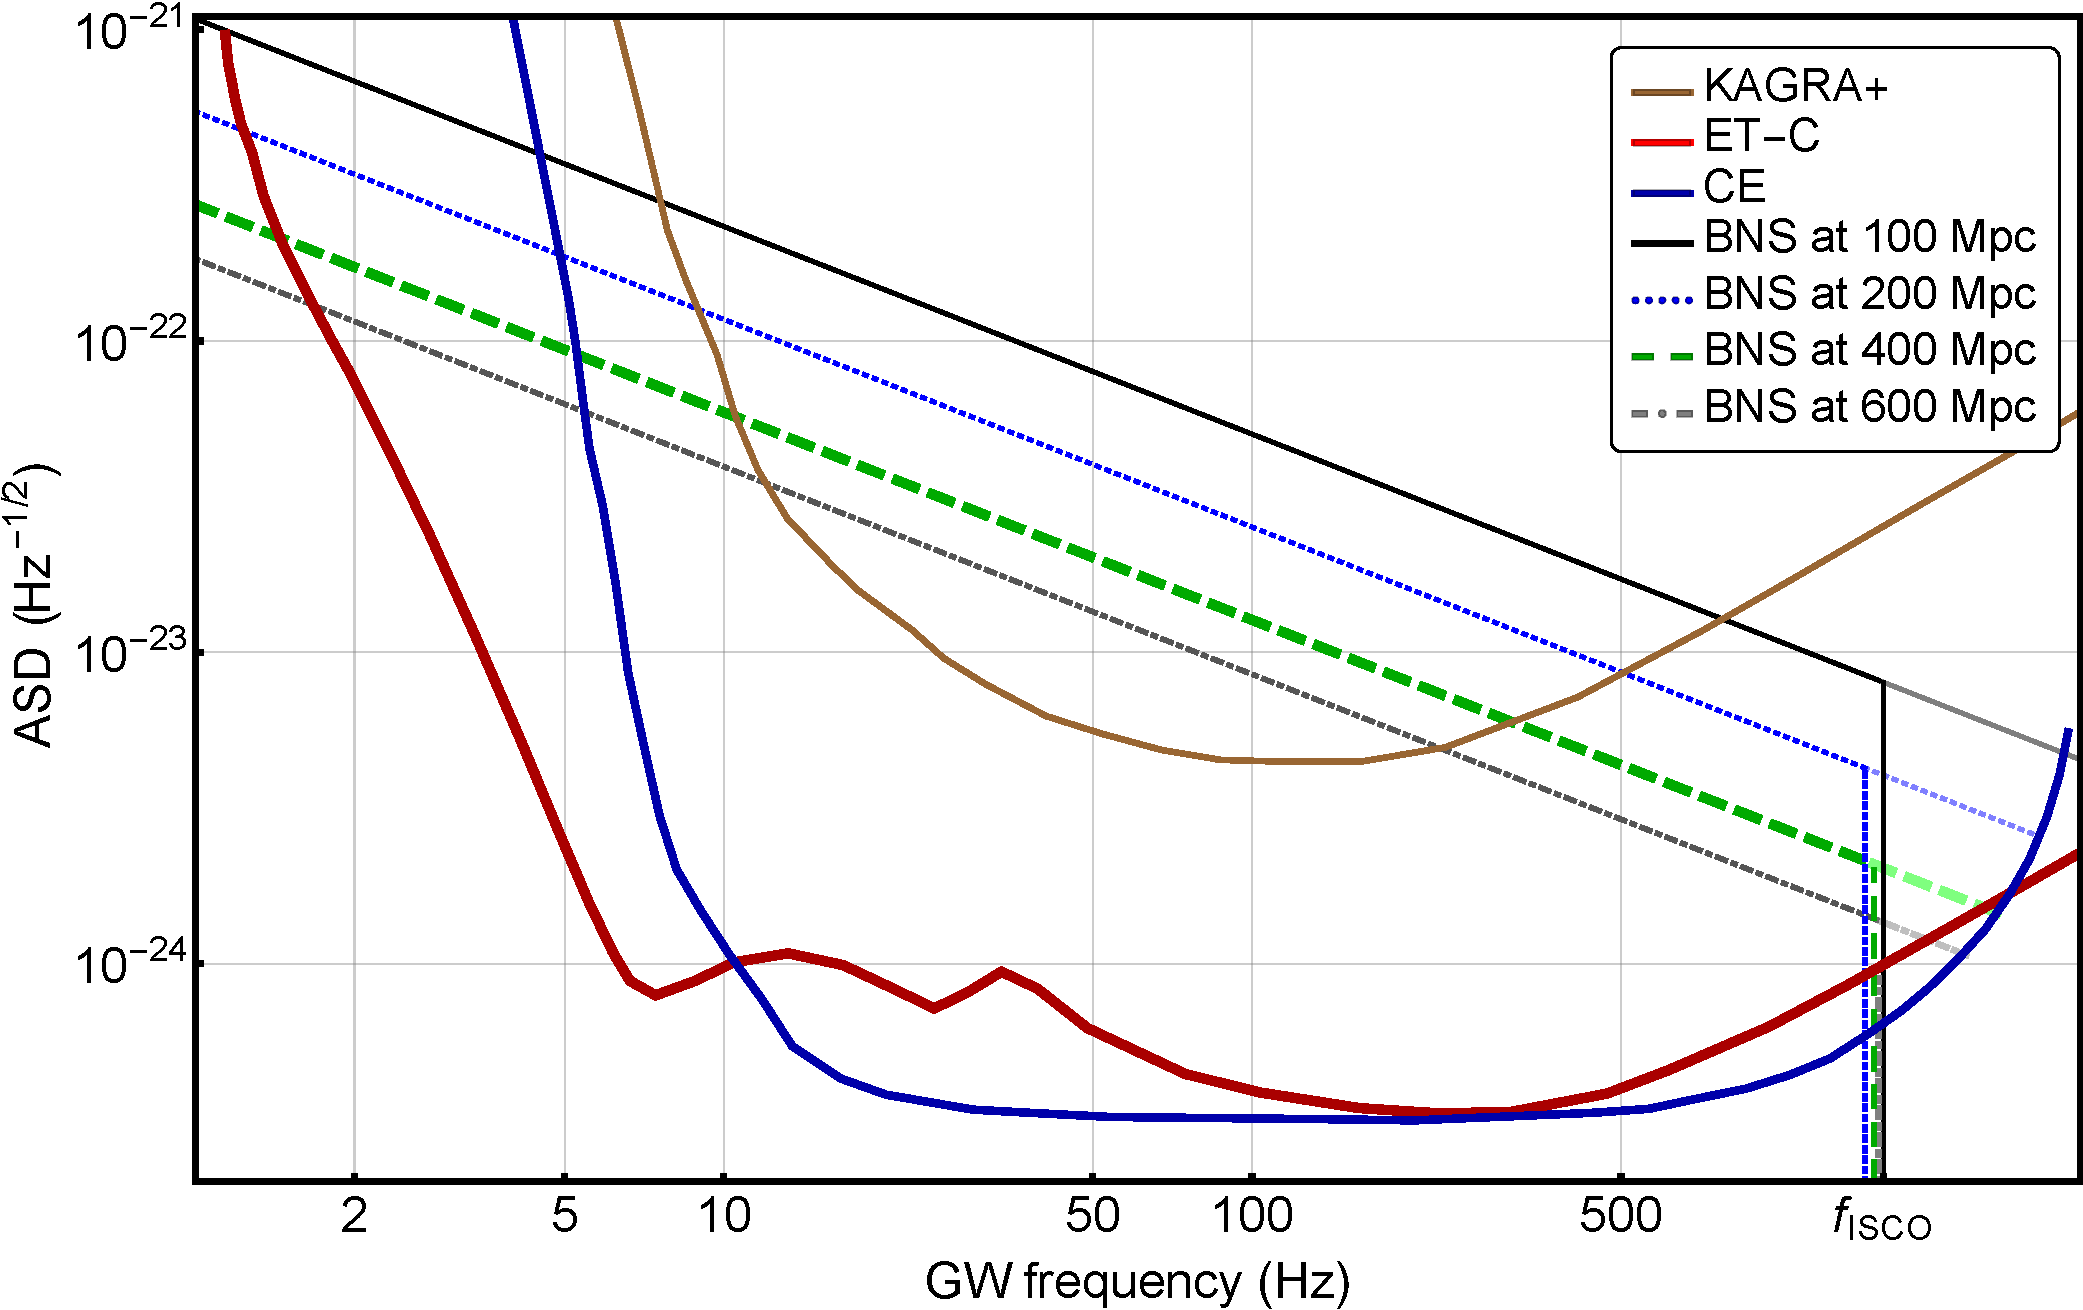
\includegraphics[width=\linewidth]{../Figs/ET_strains_redshifted.pdf}
\caption{Typical GW sources that may be harbingers of GRBs in the 2030s: $1.4 M_\sun-1.4 M_\sun$ inspiralling BNS systems sweeping across 
the Einstein Telescope's sensitivity band for both B and C configurations.
The solid (black), dotted (blue), dashed (green), and dot-dashed lines (gray) lines are the redshift-corrected
RMS-averaged strains, $2\sqrt{f}\tilde{H}_\text{ET}$, at luminosity distances of $D=100, 200, 400, 1000\,$Mpc, respectively. 
The vertical lines with correspondingly identical patterns (colors) mark the redshifted ISCO frequencies $(1+z)^{-1} f_\text{ISCO}$ at which point we terminate each inspiral.
As the true ISCO frequency is likely larger than $f_\text{ISCO}$ cite{Marronetti:2003hx}, the inspirals would continue to nearly 2\,kHz indicated by the 
faded lines in the plot (drawn to 5\,kHz for aesthetic reasons).
%However, numerical simulations indicate that the actual ISCO is smaller than the Schwarzschild value $6GM/c^2$ hence the true ISCO
%frequency is greater than $f_\text{ISCO}$ used here.
%As shown, Einstein Telescope is sensitive enough to accumulate more SNR in this $f>f_\text{ISCO}$ regime.
%Once again, keep in mind that we artificially extended the leading-order $f^{-2/3}$ power law past $f\sim 100\,$Hz at which point tidal effects actually visibly modify this behavior.
}
\label{fig:ETB2030}
\end{figure*}

\begin{acknowledgements}
 SA thanks
\end{acknowledgements}


\end{document}
